\documentclass[journal]{IEEEtran}
%\documentclass[12pt, draftclsnofoot, onecolumn]{IEEEtran}
\newcommand{\D}{\displaystyle}
% If the IEEEtran.cls has not been installed into the LaTeX system files,
% manually specify the path to it:
%\documentclass[journal]{../sty/IEEEtran}
%%%%%%%%%%%%%%%%%%%%%%%%%%%%%%%%%%%%%%%%%%%%%%%%%%%%%%%%%%%%%%%%%%%%%%%%%%%%%%%%%%%%%%%%%%
%%%%%%%%%%%%%%%%%%%%%%%%%%%%%%%%%%%%%%%%%%%%%%%%%%%%%%%%%%%%%%%%%%%%%%%%%%%%%%%%%%%%%%%%%%
%\usepackage[switch]{lineno} %
\usepackage{color}
\definecolor{orange}{RGB}{255,165,0}
\usepackage{multirow}
\usepackage{graphicx}
\usepackage{psfrag}
\usepackage{amsmath}
\usepackage{graphicx}
\usepackage{booktabs}
\usepackage{enumerate}
\usepackage{cite}
\usepackage{mathrsfs,amssymb}
%\usepackage{float}
\usepackage{floatrow}
\usepackage{stfloats}
\usepackage[section]{placeins}%
%%%%%%%%%%%%%%%%%%%%%%%%%%%%%%%%%%%%%%%%%%%%%%%%%%%%%%%%%%%%%%%%%%%%%%%%%%%%%%%%%%%%%%%%%%
%%%%%%%%%%%%%%%%%%%%%%%%%%%%%%%%%%%%%%%%%%%%%%%%%%%%%%%%%%%%%%%%%%%%%%%%%%%%%%%%%%%%%%%%%%
\usepackage{dsfont}
\usepackage{multirow}
\usepackage{psfrag}
\usepackage{amsmath}
\usepackage{booktabs}
\usepackage{enumerate}
\usepackage{cite}
\usepackage{mathrsfs,amssymb}
\usepackage{epstopdf}
\usepackage{diagbox}
\usepackage{lettrine}
\usepackage{caption}
\usepackage{booktabs}
\usepackage{makecell}
\usepackage{amsmath}
%%%%%%%%%%%%%%%%%%%%%%%%%%%%
\makeatletter
\newif\if@restonecol
\makeatother
\let\algorithm\relax
\let\endalgorithm\relax
\usepackage[linesnumbered,ruled,vlined]{algorithm2e}%[ruled,vlined]{
\usepackage{algpseudocode}
\usepackage{amsmath}
\renewcommand{\algorithmicrequire}{\textbf{Input:}}  % Use Input in the format of Algorithm
\renewcommand{\algorithmicensure}{\textbf{Output:}} % Use Output in the format of Algorithm
%%%%%%%%%%%%%%%%%%%%%%%%%%
\usepackage{array}

\hyphenation{op-tical net-works semi-conduc-tor}

%% FENYE
\makeatletter
\newenvironment{breakablealgorithm}
  { \begin{breakablealgorithm}
   \begin{center}
     \refstepcounter{algorithm}% New algorithm
     \hrule height.8pt depth0pt \kern2pt% \@fs@pre for \@fs@ruled
     \renewcommand{\caption}[2][\relax]{% Make a new \caption
       {\raggedright\textbf{\ALG@name~\thealgorithm} ##2\par}%
       \ifx\relax##1\relax % #1 is \relax
         \addcontentsline{loa}{algorithm}{\protect\numberline{\thealgorithm}##2}%
       \else % #1 is not \relax
         \addcontentsline{loa}{algorithm}{\protect\numberline{\thealgorithm}##1}%
       \fi
       \kern2pt\hrule\kern2pt
     }
  }{ \end{breakablealgorithm}
     \kern2pt\hrule\relax% \@fs@post for \@fs@ruled
   \end{center}
  }
\makeatother
%%%%%%%%%%%%%%%%%%%%%%%%%%%

\begin{document}

\title {\textcolor{blue}{ADP-based for Robust Decentralized \textcolor{orange}{Load Frequency Control} Schemes to  Multi-area Asynchronous Markov Jumping Power Systems with Experience Replay}
	\footnote{ }
\author{Hai Wang, Jun Cheng, Shengda Tang, Iyad Katib, Xuan Qiu}%\textit{Fellow, IEEE}
}
\date{}
\maketitle
\normalsize

%%%%%%%%%%%%%%%%%%%%%%%%%%%%%%
\section{Case Study 1}	

In this section, we give a special case to simulate and verify the effectiveness of the algorithm to solve zero-sum games for LFC with Markov jumping parameter. We do not consider the area interconnection case and only consider the LFC control problem for a single-area Markov jumping power system.

The  power system under consideration is assumed to have two operating ranges denoted by  $\mathcal{M} = \{1,2\}$  representing ``Nominal load" and ``Heavy load", respectively. The power system is supposed to jump stochastically between the two modes, and the system parameter values for each mode are shown in the Table \ref{table2}.
The corresponding transition rate matrix of the two system modes is given as
\begin{align*}
    \Pi=\left[ \begin{matrix}
        -3.6&		3.6\\
       1.0&		-1.0\\
    \end{matrix} \right].
\end{align*}
%%%%%%%%%%%%%%%%%%%%%%%%%
Moreover, the weight matrices are defined as $Q_{1}=Q_{2}=diag[1,0.1,0.1,1]$, $R_{1}=R_{2}=0.01$. Choose the initial controller gain $K^{(0)}_m$ and the external disturbance gain $L^{(0)}_m$ arbitrarily, without loss of generality, and we choose $K^{(0)}_{1}=K^{(0)}_{2}=0$, $L^{(0)}_{1}=L^{(0)}_{2}=0$. While the corresponding eigenvalue of $(\mathbf{A}_{m}-B_{m }K^{(0)}_{m}+F_{m }L^{(0)}_{m})$ are listed in Table \ref{table3}, from which we can see that the system will become unstable since the system is not Hurwitz.
%%%%%%%%%%%%%%%%%%%%%%%%%%%%%%%%%
\begin{table}[htbp]
	\centering
	\fontsize{8}{10}\selectfont
	\caption{Value of system parameter under different operating conditions}\label{table2}
	\begin{tabular}{l|l|l|l}
	\hline
	\multicolumn{2}{c}{ Nominal load ( $m=1$)}  &  \multicolumn{2}{|c}{ Heavy load ( $m=2$)}  \\
	\cline{1-2}
	\cline{3-4}
	Parameter & Value & Parameter & Value  \\
	\hline
	$T_{g1}$  &   0.073     &    $T_{g2}$     &    0.144    \\
	$T_{t1}$  &  0.273      &    $T_{t2}$     &    0.535    \\
	$T_{p1}$  &   15.037    &    $T_{p2}$     &    18.75   \\
	$K_{p1}$  &   120.3     &    $K_{p2}$     &   150.4     \\
	%$T_{p}(1)$  &   0.278     &    $T_{p}(2)$     &   0.375     \\
	$\tilde{R}_1$      &   2.0       &    $\tilde{R}_2$         &    1.5      \\
	$K_{e1}$  &   0.6       &    $K_{e2}$     &   0.8       \\
	\hline
	\end{tabular}
	\end{table}	
%%%
\begin{table}[H]%[htbp]
	\newcommand{\tabincell}[2]{\begin{tabular}{@{}#1@{}}#2\end{tabular}}
	\renewcommand{\arraystretch}{1.5}
	\centering
	\fontsize{8}{10}\selectfont
 %\fontsize{8}{12}\selectfont
	\caption{Initial gain pairs and  corresponding eigenvalues }  %
	\label{table3}  %
	\begin{tabular}{c|cc}
\Xhline{1pt}
\multicolumn{1}{c}{$m $}{\vline}& \multicolumn{1}{c}{Initial $(K_{m }^{(0)},L_{m }^{(0)})$ }&\multicolumn{1}{l}{$\sigma(\mathbf{A}_{m}^{(0)}-B_{m}K^{(0)}_{m }+F_{m}L^{(0)}_{m})$}\\
     \hline
 	\multicolumn{1}{c}{$1$}{\vline}& \multicolumn{1}{l}{ \tabincell{c}{$K^{(0)}_{1}=[0,0,0,0]$\\$L^{(0)}_{1}=[0,0,0,0]$}
	}&
 	\multicolumn{1}{l}{$\left[ \begin{matrix} -16.2586 + 0.0000i\\
		~1.5529 + 0.0000i\\
	   -4.9612 + 3.1476i\\
	   -4.9612 - 3.1476i  \\\end{matrix} \right]$ }
\\
\Xcline{1-3}{0.5pt}
	\multicolumn{1}{c}{$2$}{\vline}& \multicolumn{1}{l}{\tabincell{c}{$K^{(0)}_{2}=[0,0,0,0]$\\$L^{(0)}_{2}=[0,0,0,0]$}}&
 	\multicolumn{1}{l}{$\left[ \begin{matrix} -5.4464 + 1.2859i\\
		-5.4464 - 1.2859i\\
		-0.2974 + 0.0000i\\
		~~ 0.3233 + 0.0000i \\\end{matrix} \right]$ }
\\
\Xhline{1pt}			
	\end{tabular}
\end{table}

Now, let $r_{0}=1$, $x(0)=[0.1,-0.1,0.1,-0.1]^{T}$. We simulate the model from $t = 0$ to $t = 10$ sec.
All the parameters of the power system, except for the transition rate matrix, are assumed to be unknown. We inject the noises given as
\begin{align*}
e_{1}&=\sum_{k=1}^{100}{\left( 0.1e^{-0.01t}\sin \left( \omega _kt \right) +0.5\cos \left( \omega _kt \right) \right)},\\ e_{2}&=e^{-0.01t}+\sum_{k=1}^{100}{\sin \left( \omega _kt \right)},
\end{align*}
where $ \omega_{k}$, $ k=1,2, \ldots, 100$, are random numbers uniformly distributed on $[-50,50]$.

Using the proposed Algorithm 1, we obtain the stabilizing gain pair $({K}_{m}^{(\kappa)},{L}_{m}^{(\kappa)})$ as follows:
\begin{align*}
	{K}^{(\kappa)}_{1}&=[14.3241~ 14.2643 ~ 4.0943~ 12.3167],\\
	{K}^{(\kappa)}_{2}&=[19.5322~   25.6232~ 4.0504~ 23.1600],\\
	{L}^{(\kappa)}_{1}&=[-0.1827 ~ -0.1213 ~ -0.0068 ~ -0.1856],\\
	{L}^{(\kappa)}_{2}&=[-0.3172~   -0.2978~   -0.0184~  -0.4462],
\end{align*}
and the corresponding eigenvalue is
\begin{align*}
	\sigma(\mathbf{A}_{1}^{(\kappa)}-B_{1}{K}^{(\kappa)}_{1}+F_{1}{L}^{(\kappa)}_{1})
	=&\left[ \begin{matrix}  -75.9512 + 0.0000i\\
		-1.0840 + 4.3238i\\
		-1.0840 - 4.3238i\\
		-1.1335 + 0.0000i \end{matrix} \right],\nonumber\\
	\sigma(\mathbf{A}_{2}^{(\kappa)}-B_{2}{K}^{(\kappa)}_{2}+F_{2}{L}^{(\kappa)}_{2})
	=&\left[ \begin{matrix}   -32.9413 + 0.0000i\\
		-1.2773 + 4.9580i\\
		-1.2773 - 4.9580i\\
		-0.9617 + 0.0000i\end{matrix} \right],	
\end{align*}
which implies that the gain pair $({K}_{m}^{(\kappa)},{L}_{m}^{(\kappa)})$  is Hurwtiz.

In this simulation scenario, the number of iteration is 36 and 139 respectively, and the process of changing the real part of the eigenvalues is illustrated in Fig. \ref{fig:1}-\ref{fig:2}. In addition, in the case of unknown dynamics, the parameters $\beta_{1}$, $\beta_{2}$ are both set to $20$ and the end of the process of finding a stabilizing initial value is marked before the parameter $\rho^{(k)} _{m}$ becoming negative, see Fig. \ref{fig:3}-\ref{fig:4} for details of the change in the real part.

 \begin{figure} %[H]
	\centering
	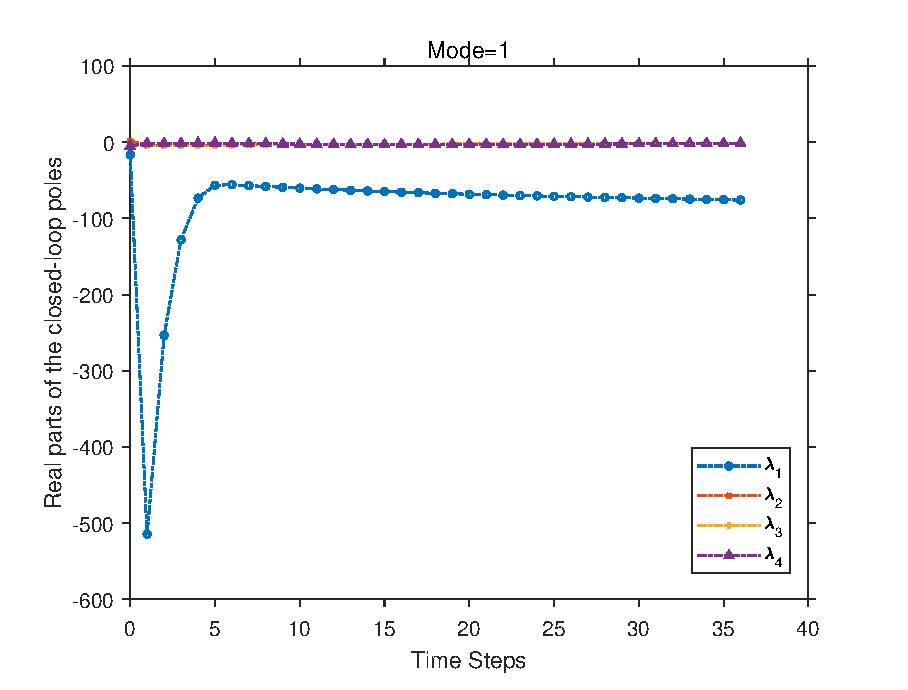
\includegraphics[scale=0.6]{mode1_eig.eps}
	\caption{Real parts of the closed-loop poles  via Algorithm 1 in mode 1.}
	\label{fig:1}
	\end{figure}


 \begin{figure} %[H]
	\centering
	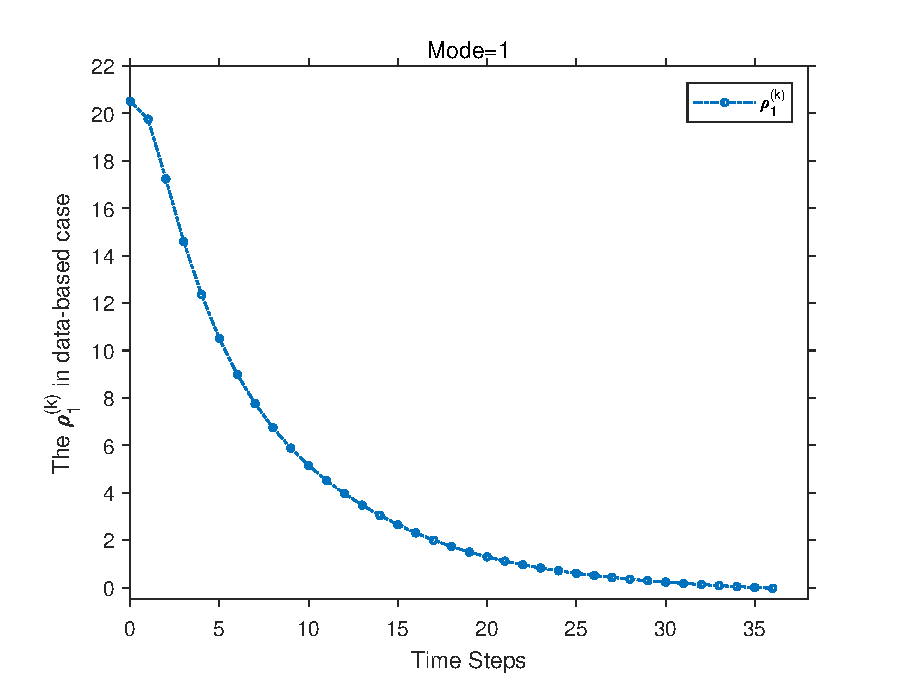
\includegraphics[scale=0.6]{rho1.eps}
	\caption{Trend of $\rho^{(k)} _{1 }$ via Algorithm 1 in mode 1.}
	\label{fig:2}
	\end{figure}

\begin{figure} %[H]
	\centering
	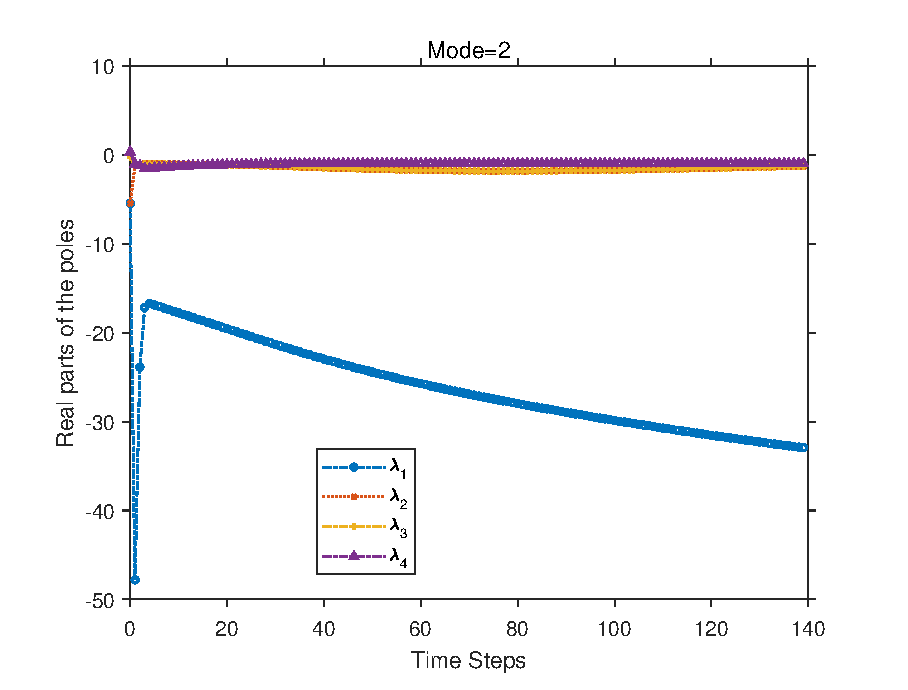
\includegraphics[scale=0.6]{mode2_eig.eps}
	\caption{Real parts of the closed-loop poles  via Algorithm 1 in mode 2.}
	\label{fig:3}
	\end{figure}
	
	
\begin{figure} %[H]
    \centering
    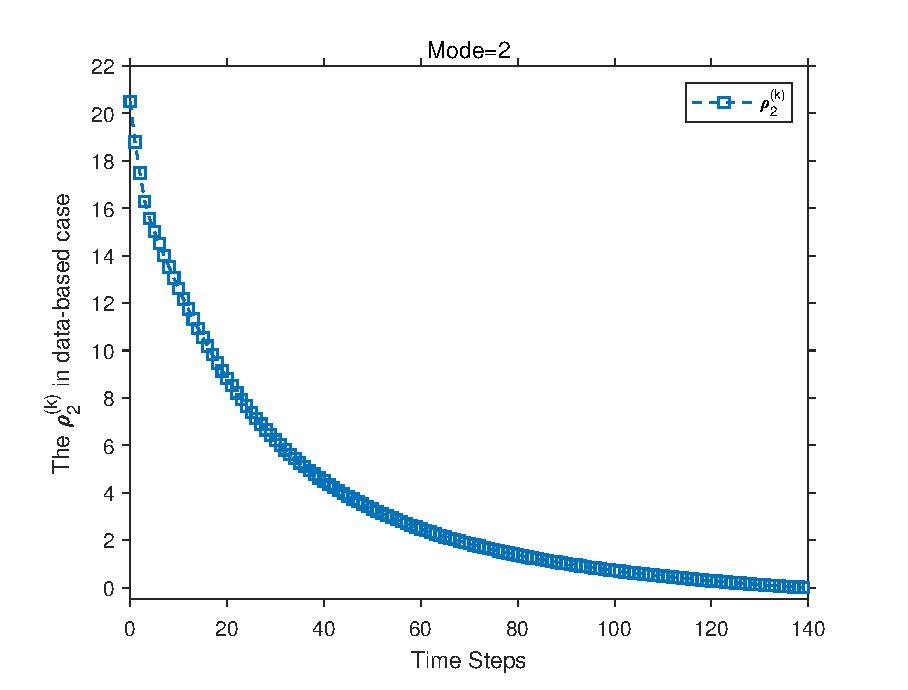
\includegraphics[scale=0.6]{rho2.eps}
	\caption{Trend of $\rho^{(k)} _{2 }$ via Algorithm 1 in mode 2.}
	\label{fig:4}
\end{figure}	

\begin{table*}[htbp]
	\renewcommand{\arraystretch}{1.5}
	\centering  %
 \fontsize{8}{10}\selectfont
	\caption{Comparison between the results obtained by \cite{se1whn} and the those obtained by Algorithm 1}
	\label{table4}
\begin{tabular}{c|cc}
\Xhline{1pt}
\multicolumn{1}{c}{$m$}{\vline}& \multicolumn{1}{c}{Obtained by {\cite{se1whn}}}&\multicolumn{1}{c}{Obtained by Algorithm 1}\\
  \hline
\multicolumn{1}{c}{$1$}{\vline}&
\multicolumn{1}{l}{ $P_{1}^{*}=\begin{bmatrix}	
		0.23818523 &  0.15962699 &  0.01060335 &  0.20360638\\
		0.15962699 &  0.16691434 &  0.01169301 &  0.13199525\\
		0.01060335 &  0.01169301 &  0.00258429 &  0.00788275\\
		0.20360638 &  0.13199525 &  0.00788275 &  1.58693045
		 \end{bmatrix}$}&
	  \multicolumn{1}{l}{ $P_{1}^{(15)}= \begin{bmatrix}	
		0.23818523 &  0.15962699  & 0.01060335 &   0.20360637\\
		0.15962699 &  0.16691434 &  0.01169301 &   0.13199525\\
		0.01060335  & 0.01169301 &  0.00258429 &   0.00788275\\
		0.20360637 &  0.13199525 &  0.00788275 &   1.58693045
	 \end{bmatrix} $ }\\
 \Xcline{1-3}{0.5pt}
 %%%%%%%%%%%%%%%%%%%%%%%%%%%%%%%%%%%%%%%%%%%%%%%%%%%%%%%%%%%%%%%%%%%%%%%%%%%%%%%%%%%%%%%%%%%%%%%%%%%%%%%%%%%%%%
 \multicolumn{1}{c}{$2$}{\vline}&
 \multicolumn{1}{l}{ $P_{2}^{*}= \begin{bmatrix}	
	0.36471273 &  0.34253493 &  0.02166601 &  0.33353455\\
	0.34253493 &  0.44504765 &  0.02974324 &  0.29161237\\
	0.02166601  & 0.02974324 &  0.00532798 &  0.01646038\\
	0.33353455  & 0.29161237 &  0.01646038 &  1.63287855
 \end{bmatrix} $ }&
   \multicolumn{1}{l}{ $P_{2}^{(15)}=\begin{bmatrix}	
	0.36471273 &  0.34253493 &  0.02166601 &  0.33353454\\
	0.34253493 &  0.44504765 &  0.02974324 &  0.29161237\\
	0.02166601  & 0.02974324  & 0.00532798 &  0.01646037\\
	0.33353454  & 0.29161237 &  0.01646037 &  1.63287854
  \end{bmatrix} $ } \\
%%%%%%%%%%%%%%%%%%%%%%%%%%%%%%%%%%%%%%%%%%%%%%%%%%%%%%%%%%%%%%%%%%%%%%%%%%%%%%%%%%%%%%%%%%%%%%%%%%%%%%%%%%%%%%
\Xhline{1pt}
\end{tabular}
\end{table*}

For comparison,  the optimal $P_{m }^{(k)}$  obtained by  Algorithm 1 and the corresponding matrices $P_{m }^{*}$ and $K_{m }^{*}$ obtained by \cite{se1whn} are listed in Table \ref{table4}, and we share the norm of the error between $P_{m }^{(k)}$ and  $P_{m }^{*}$ as follows:
\begin{align*}
\left\lVert P_{1}^{(15)}-P_{1}^{*}\right\rVert=3.7622\times 10^{-8},\\
\left\lVert P_{2}^{(15)}-P_{2}^{*}\right\rVert= 8.5152\times 10^{-9}.
\end{align*}
It is obvious that these two groups of results are consistent. The corresponding optimal policy pair  $(K_{m }^{(k)},L_{m }^{(k)})$ is shown as follows:
\begin{align*}
	{K}^{(15)}_{1}&=[14.5251 & 16.0178 &~~~~  3.5401 &  10.7983],\\
	{K}^{(15)}_{2}&=[ 15.0458 &  20.6550 &~~~~   3.7000 &  11.4308],\\
	{L}^{(15)}_{1}&=[-0.1555 &  -0.1042  &~ -0.0069 &  -0.1330],\\
	{L}^{(15)}_{2}&=[-0.2382 &  -0.2237 &~  -0.0141 &  -0.2178].
\end{align*}

Moreover, the convergence of  $P_{m }^{(k)}$  and  $K_{m }^{(k)}$  is illustrated in Fig.\ref{fig:5}-\ref{fig:8} for each corresponding mode. Fig.\ref{fig:9}-\ref{fig:10} depict the control input and external disturbance input respectively, and we can see that the power system eventually becomes stable by applying the initial gain pair $({K}_{m}^{(\kappa)},{L}_{m}^{(\kappa)})$ based on the proposed Algorithm 1.

%%%%%%%%%%%%%%%%%%%%%%%%%%%%%%%%%%%%%%%%%%%%%%
\begin{figure} %[H]
	\centering
	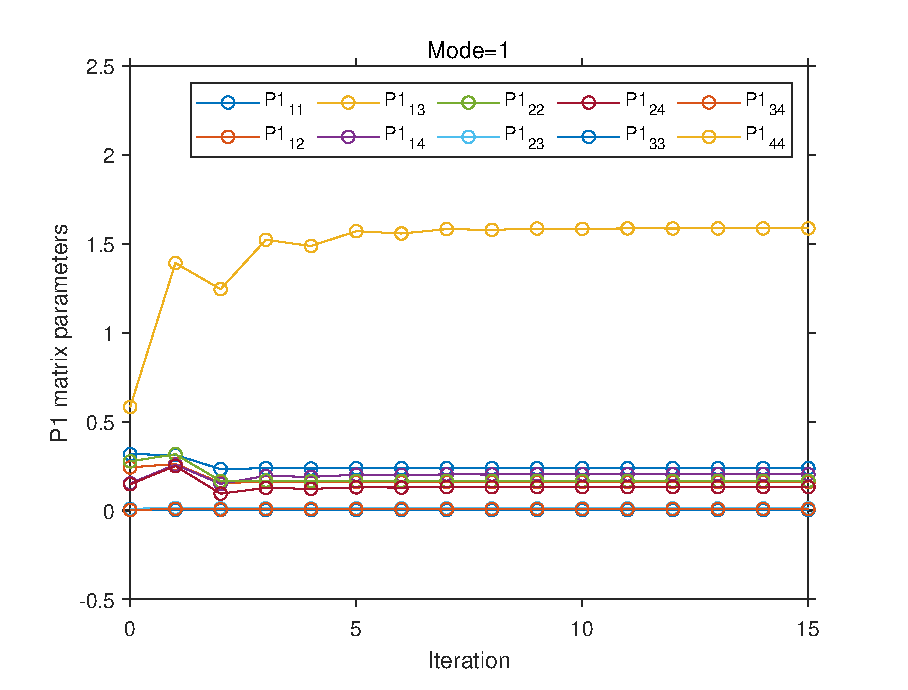
\includegraphics[scale=0.6]{elementP1mode1.eps}
	\caption{Convergence of $P_{1}$.}
	\label{fig:5}
\end{figure}

\begin{figure}%[H]
	\centering
	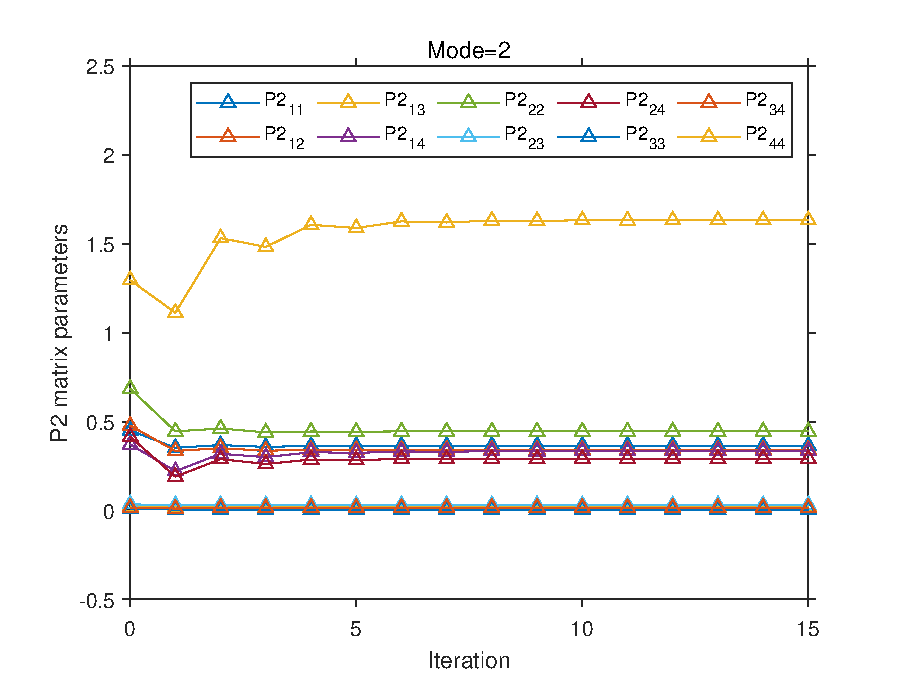
\includegraphics[scale=0.6]{elementP2mode2.eps}
	\caption{Convergence of $P_{2}$.}
	\label{fig:6}
\end{figure}

\begin{figure} %[H]
	\centering
	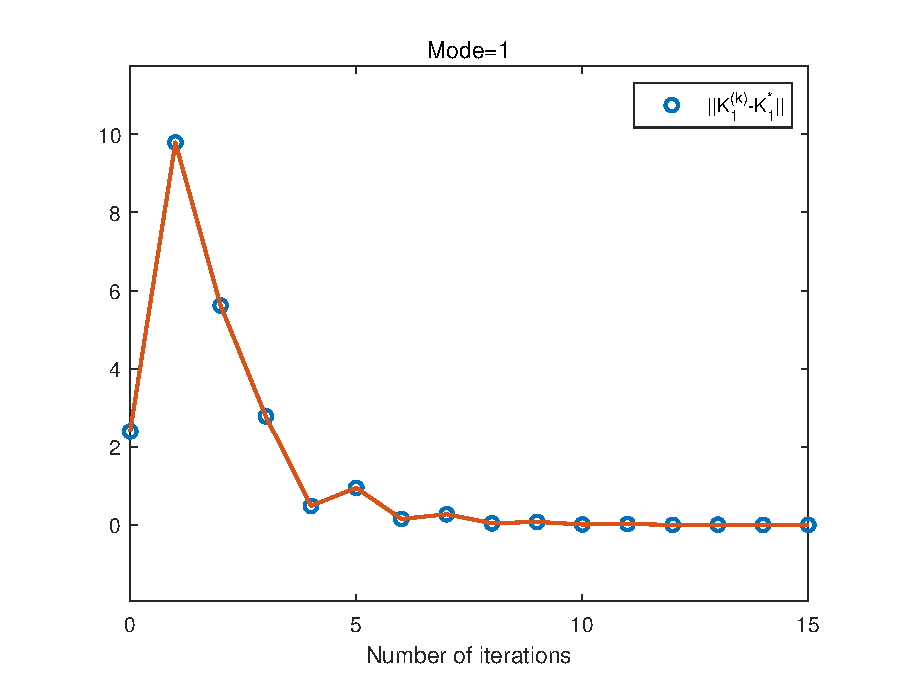
\includegraphics[scale=0.6]{optk1mode1.eps}
	\caption{Optimal $K_{1}$ in mode 1.}
	\label{fig:7}
\end{figure}

\begin{figure} %[H]
	\centering
	\includegraphics[scale=0.6]{optk2mode2.eps}
	\caption{Optimal $K_{2}$ in mode 2.}
	\label{fig:8}
\end{figure}

\begin{figure} %[H]
	\centering
	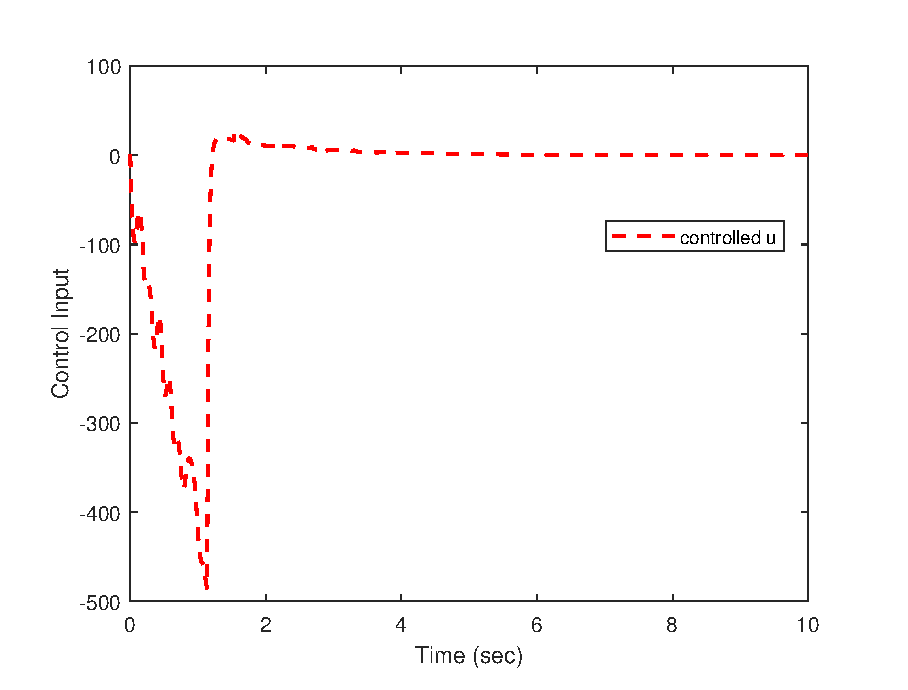
\includegraphics[scale=0.6]{2u.eps}
	\caption{Control input $u(t)$.}
	\label{fig:9}
\end{figure}

\begin{figure} %[H]
	\centering
	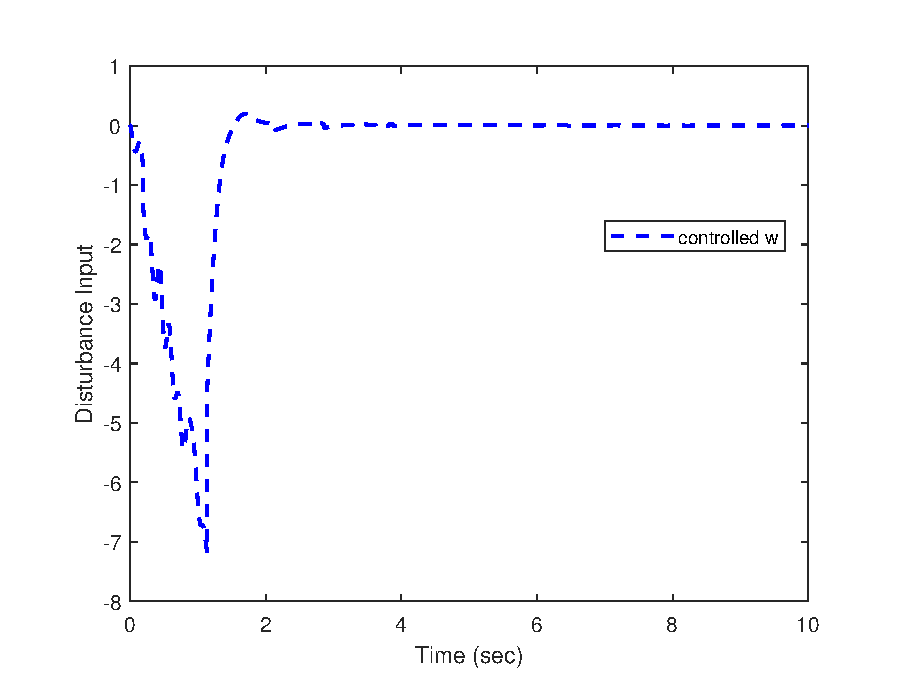
\includegraphics[scale=0.6]{2w.eps}
	\caption{Disturbance input $w(t)$.}
	\label{fig:10}
	\end{figure}
	
\begin{figure} %[H]
	\centering
	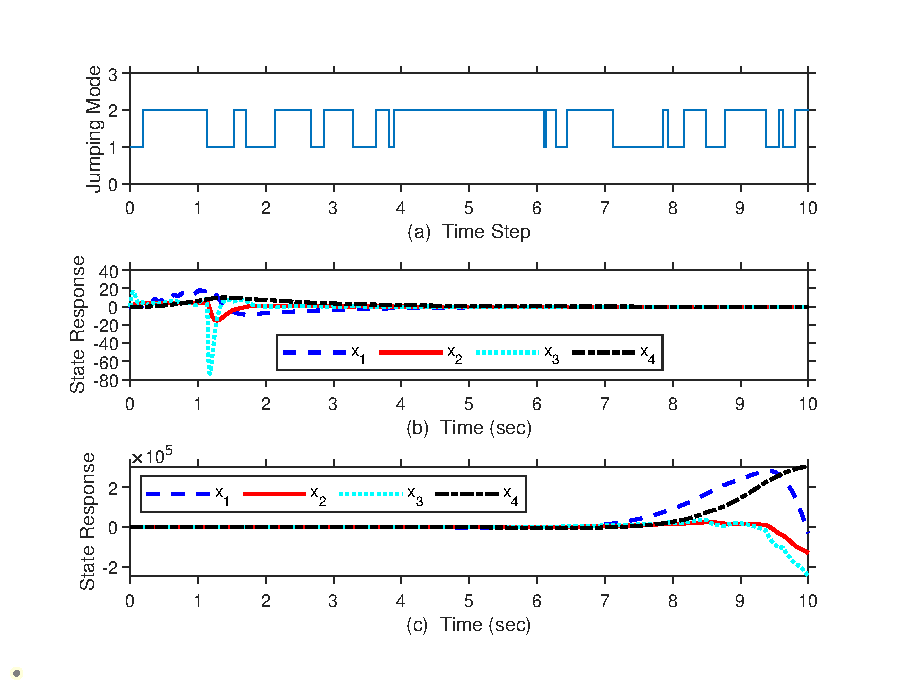
\includegraphics[scale=0.6]{2xstate.eps}
	\caption{Jumping mode $m$ and system state response of $x(t)$.}
	\label{fig:11}
\end{figure}

Now, we apply the optimal control policy and the optimal  disturbance policy obtained by Algorithm 1 to control the power system to illustrate the effectiveness of the controller designed by the proposed algorithm.

To do that, we consider two application cases. In particularly, during the first two time intervals that the mode switching occurs, a given policy pair is added to the system in both of the two cases,  however, from the moment when the third mode switching occurs to the end of the simulation, the  policy pair obtained by Algorithm 1 is applied  for one case, while  the original policy pair is still implemented in the second case.
The trajectories of the system in the two cases are plotted in Fig.\ref{fig:11}. Specially,   Fig. \ref{fig:11}(a) gives the mode evolution of the power system, Fig. \ref{fig:11}(c) describes the state trajectories of the system under the original selected control policy and disturbance policy, and the system is unstable. However, Fig. \ref{fig:11}(b) depicts the state trajectories of the system under the optimal policy pair obtained by the Algorithm 1, which implies that the proposed control algorithm is feasible and effective to control the system.




\vskip 0.5cm

\bigskip
\def\toto#1#2{\centerline{\hbox to 0.7cm{#1\hss}
\parbox[t]{15cm}{#2}}\vspace{0.2cm}}

\begin{thebibliography}{alpha}	
%%%%%%%%%%%%%%%%
\bibitem{se1whn} H.-N. Wu and B. Luo, ``Simultaneous policy update algorithms for learning the solution of linear continuous-time $\mathcal H_ {\infty}$ state feedback control ", \emph{Inf. Sci.} vol. 222, pp. 472-485, Feb. 2013.

\end{thebibliography}
			
\end{document}
			
